% !TEX root = presentation_29Jun.tex


\begin{frame}{Easter Island Mystery}
	\centering
	\begin{columns}
		\begin{column}{0.7\textwidth}
				\includegraphics[width=\linewidth]{../../EIMap_Merico2017}
			\captionof{figure}{\citet{Merico2017}}
		\end{column}
	\pause\begin{column}{0.3\textwidth}
	\centering
	\includegraphics[width=0.7\linewidth]{../../Diamond2011Cover}
	\captionof{figure}{\citet{Diamond2011}}
	\end{column}
	\end{columns}
\end{frame}

\begin{frame}{Facts of Easter Island History}
\centering
%\begin{itemize}
%	\item Forest
%	\item Polynesian Rats
%	\item Intensified deforestation from $1200\, {\rm A.D.}$ in many locations
%	\item Intensified farming (with the use of lithic mulching)
%	\item Moai statues carved between $1200$ and $1700 \, {\rm A.D.}$
%	\item European voyages arrive in $1722$, $1770$s, ... and introduce European diseases and slave trade (especially in the 19th century)
%\end{itemize}
%But: Pollen and Charcoal data is scarce and difficult to interpret.
\begin{figure}
	\centering
	\begin{subfigure}{0.15\textwidth}
	\centering
	\only<1-6>{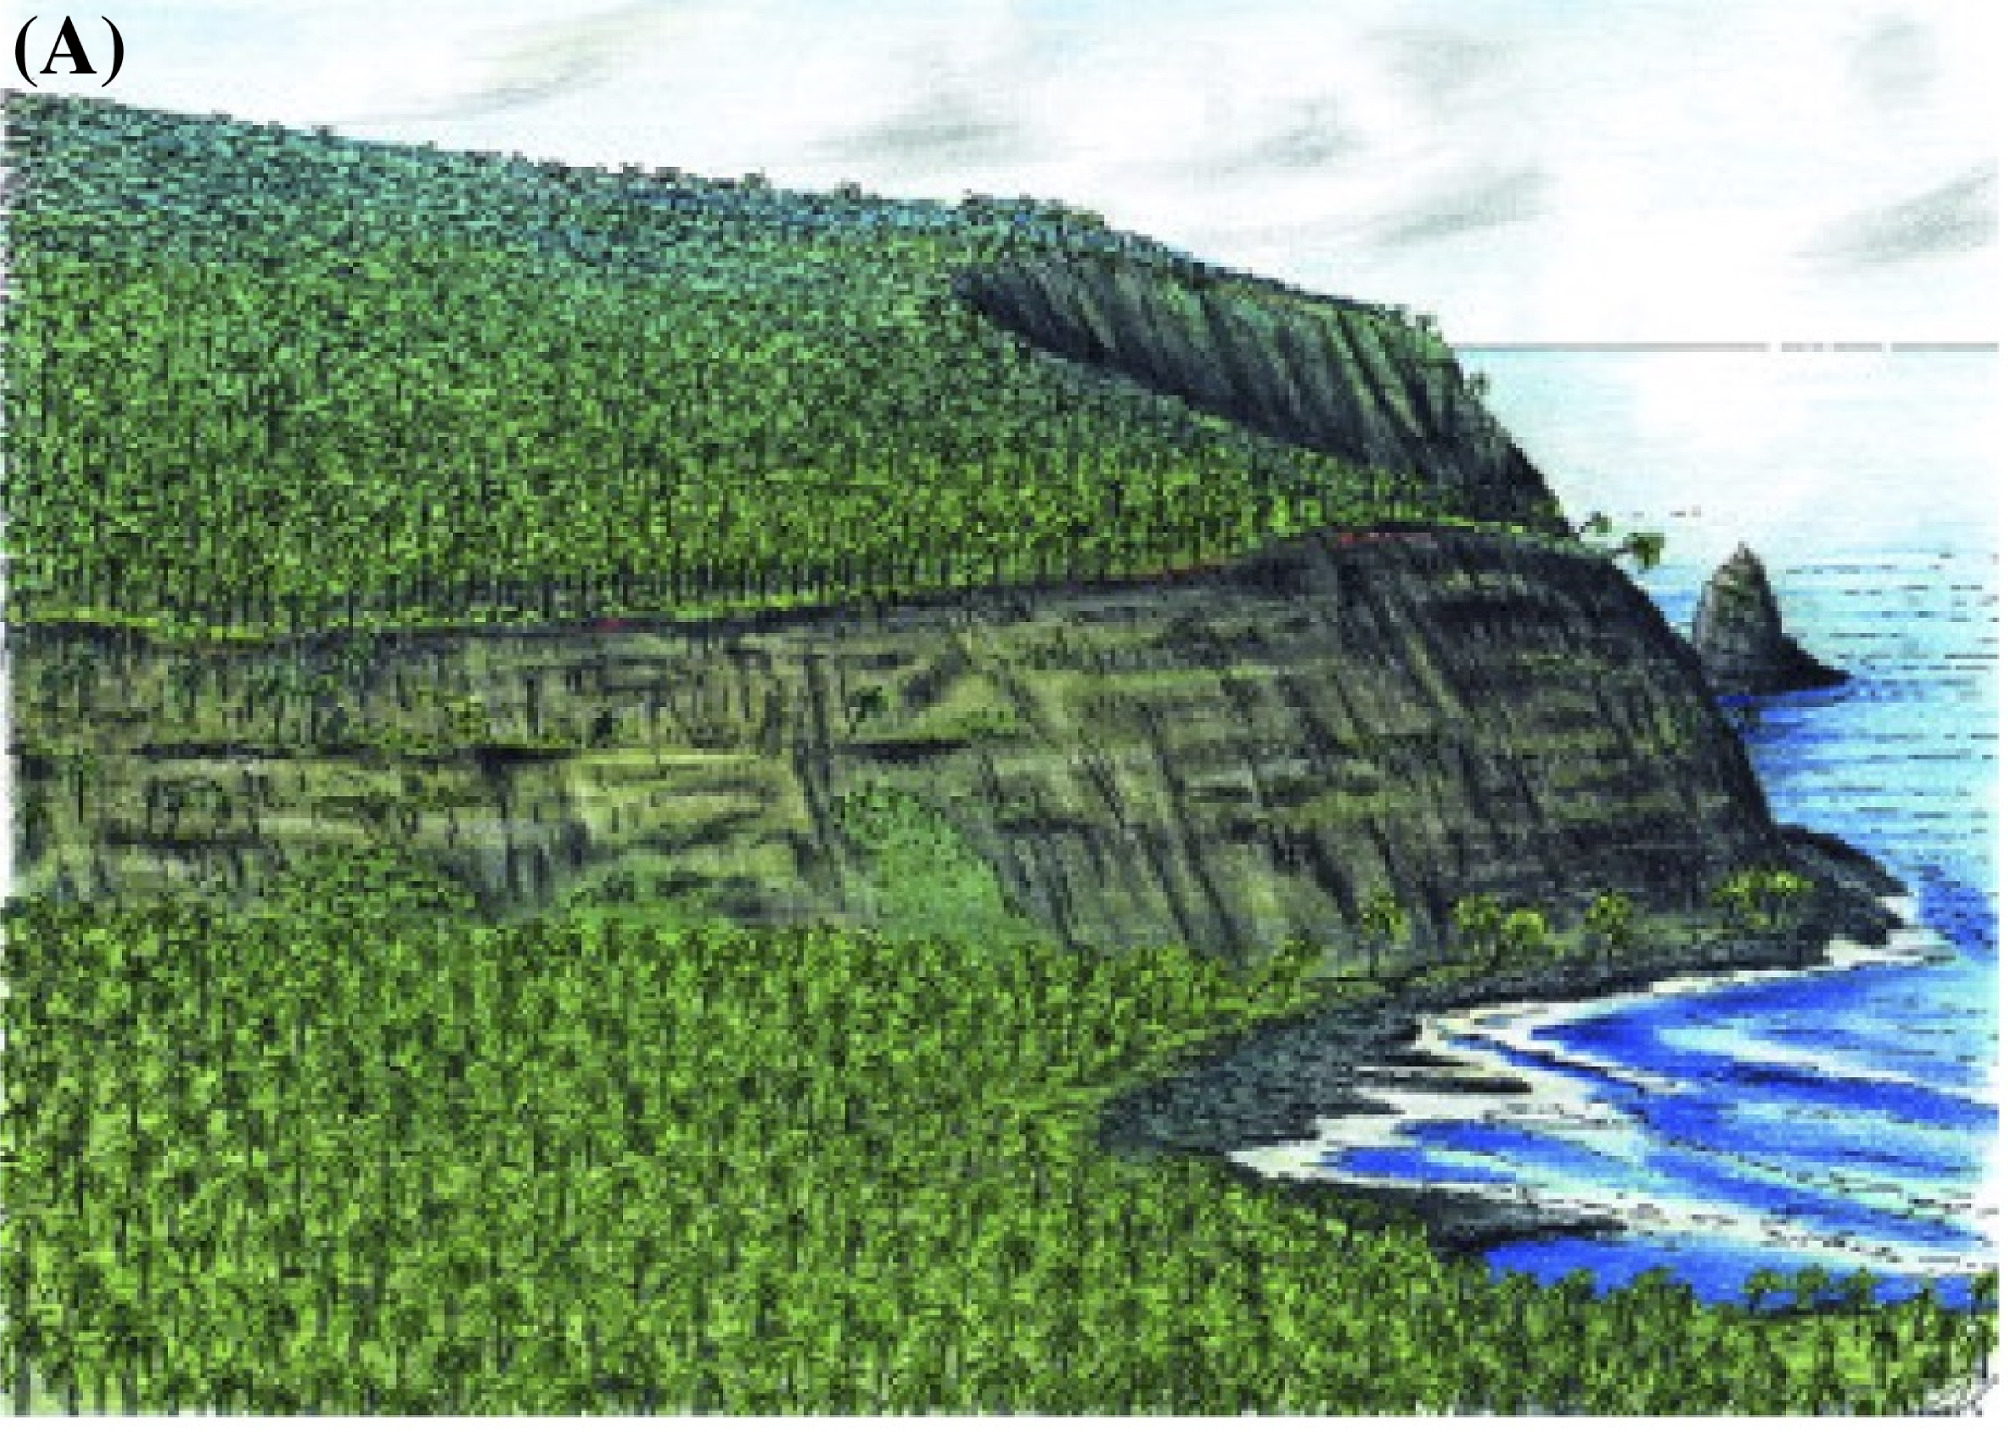
\includegraphics[height=1cm]{images/ForestGerdCloseRull2020.jpg}
	\caption{{\scriptsize Palm Forest }}}
	\end{subfigure}\hfill
	\begin{subfigure}{0.15\textwidth}
	\centering
	\only<1-6>{	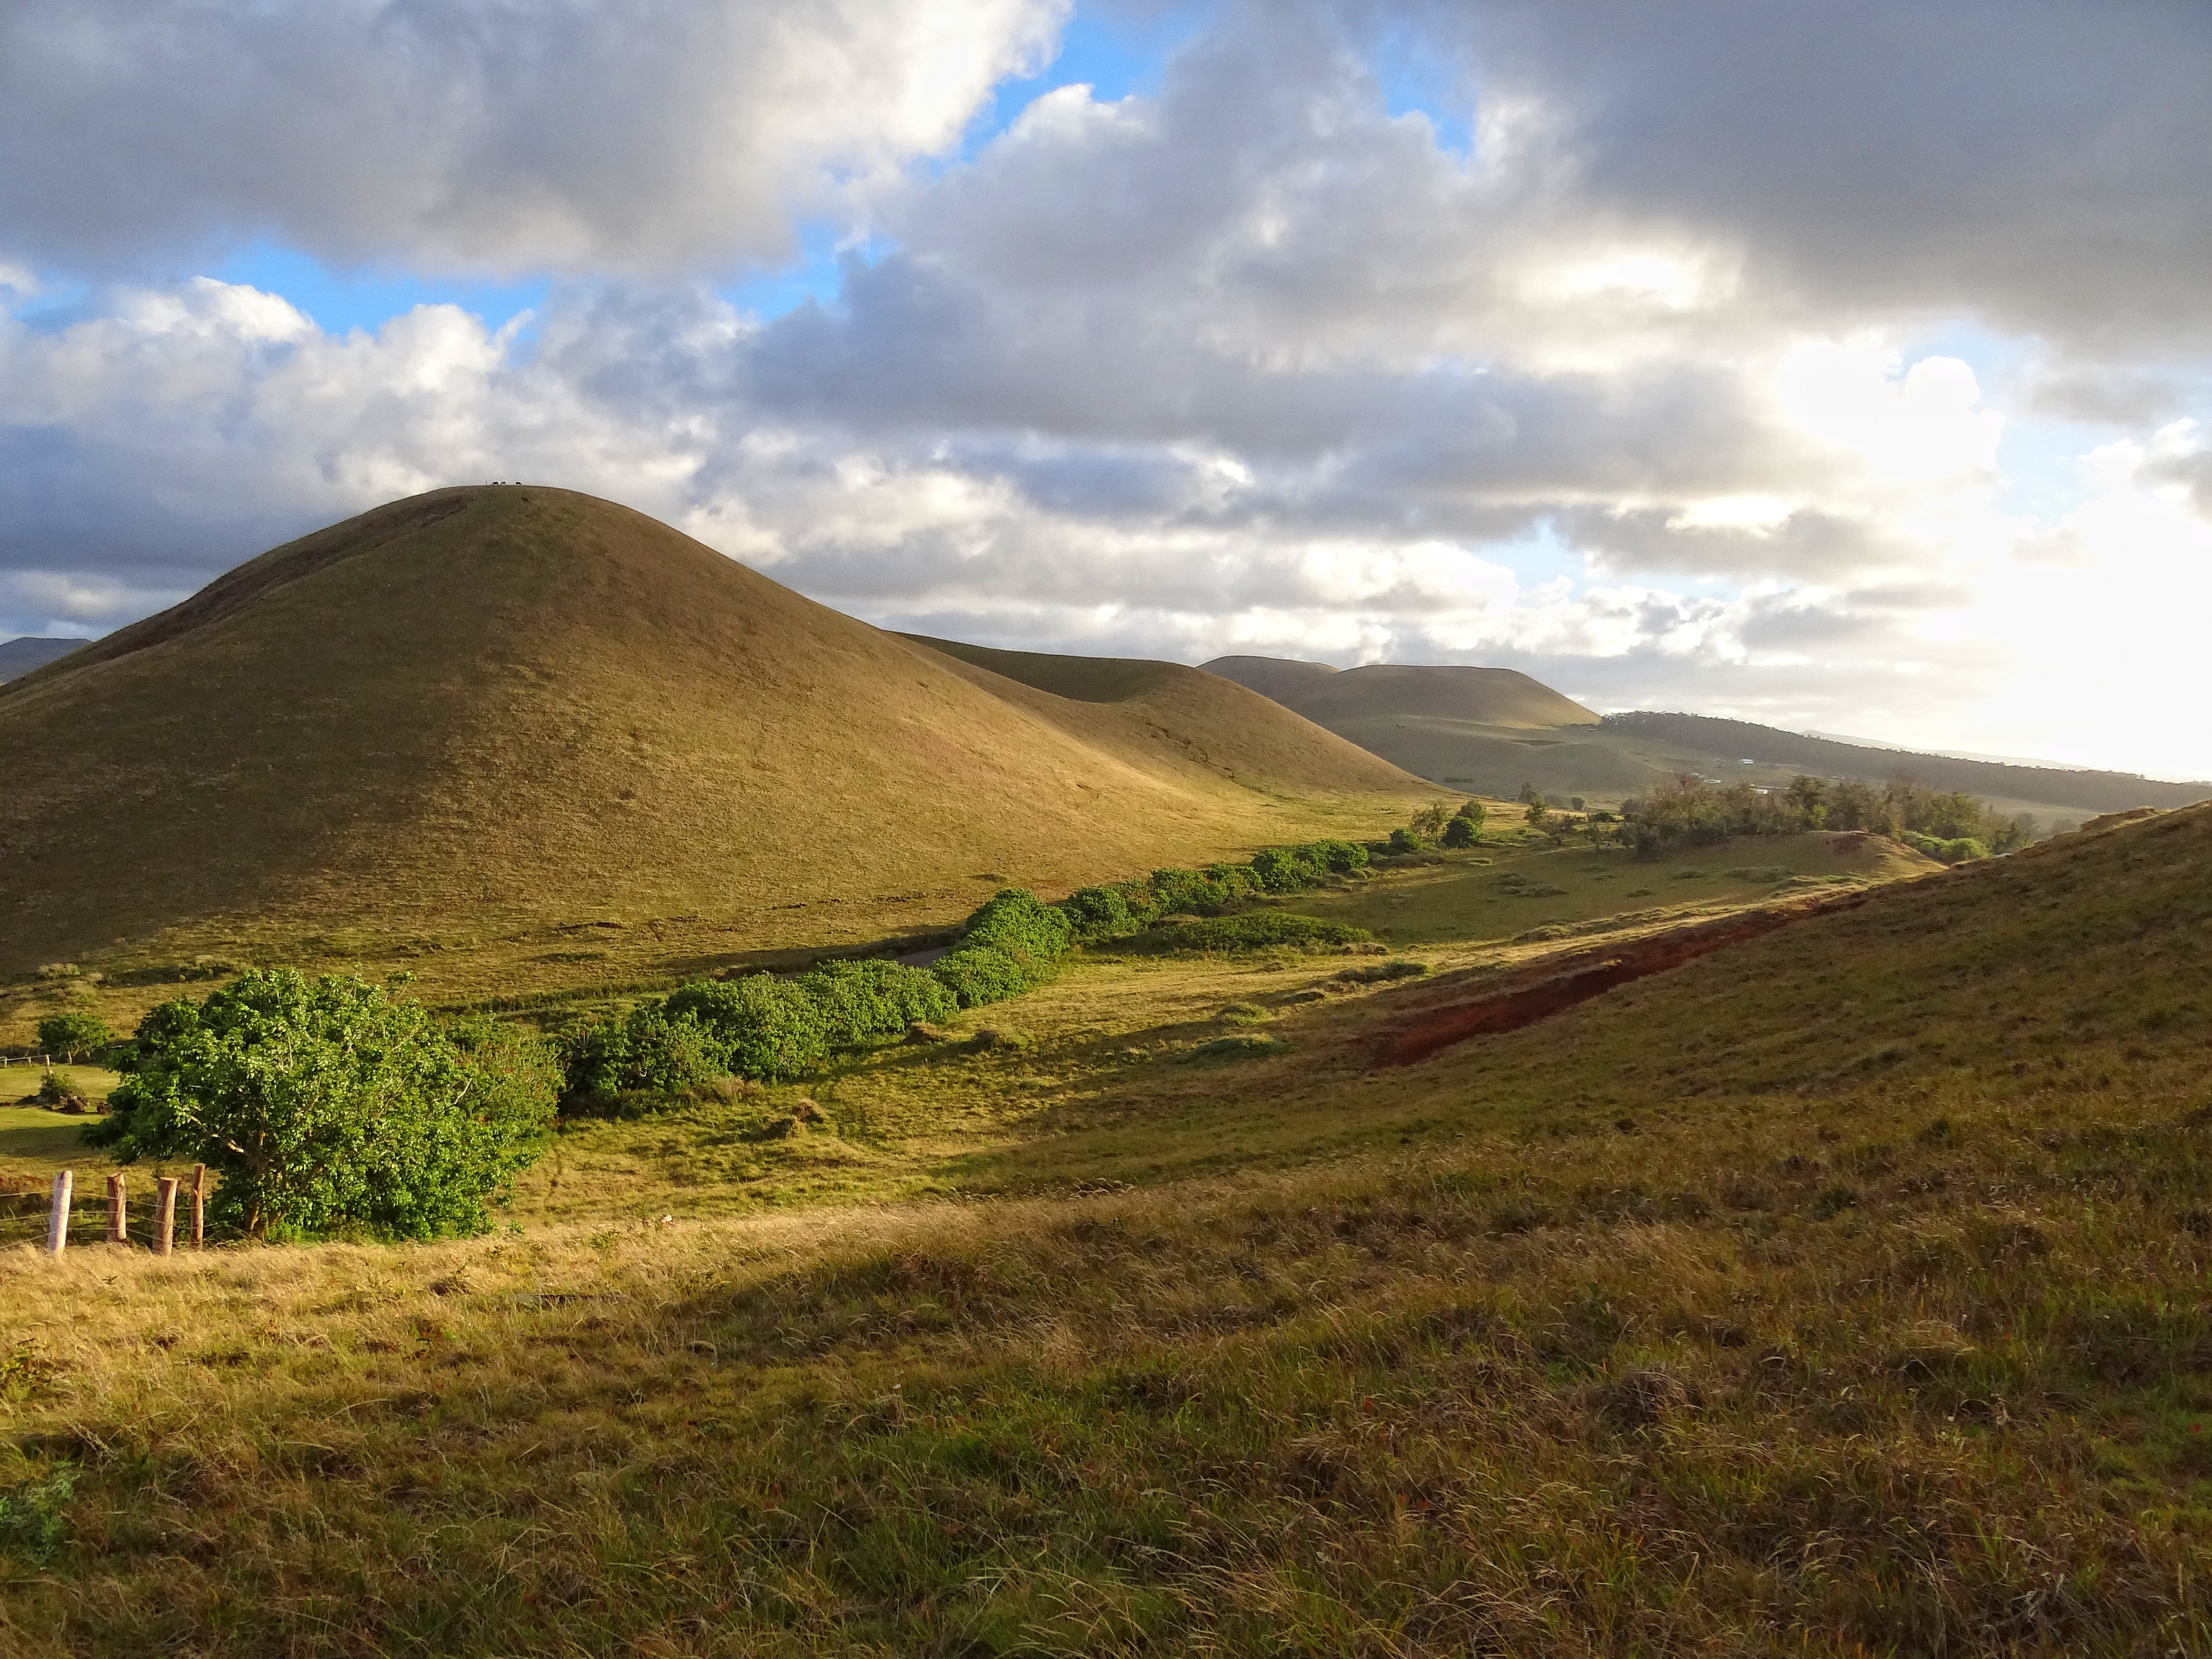
\includegraphics[height=1cm]{images/Rapa-Nui-Landscape.jpg}
	\caption{{\scriptsize Deforestation}}}
	\end{subfigure}\hfill
	\begin{subfigure}{0.15\textwidth}
	\centering
	\only<1-6>{	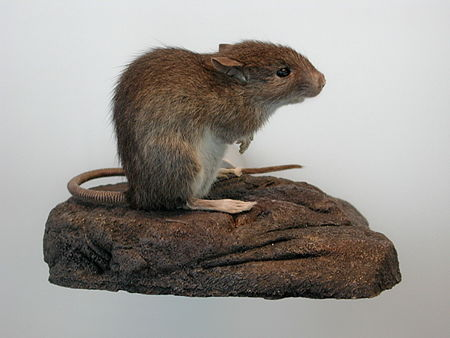
\includegraphics[height=1cm]{images/Pacific_rat.jpg}
		\caption{{\scriptsize Pacific Rats}}}
	\end{subfigure}\hfill
	\begin{subfigure}{0.15\textwidth}
	\centering
	\only<1-6>{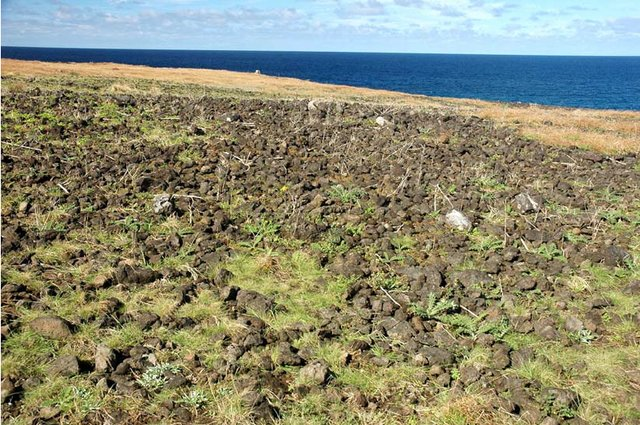
\includegraphics[height=1cm]{images/lithicMulching.jpg}
	\caption{{\scriptsize Agriculture}}}
	\end{subfigure}\hfill
	\begin{subfigure}{0.15\textwidth}
	\centering
	\only<1-6>{	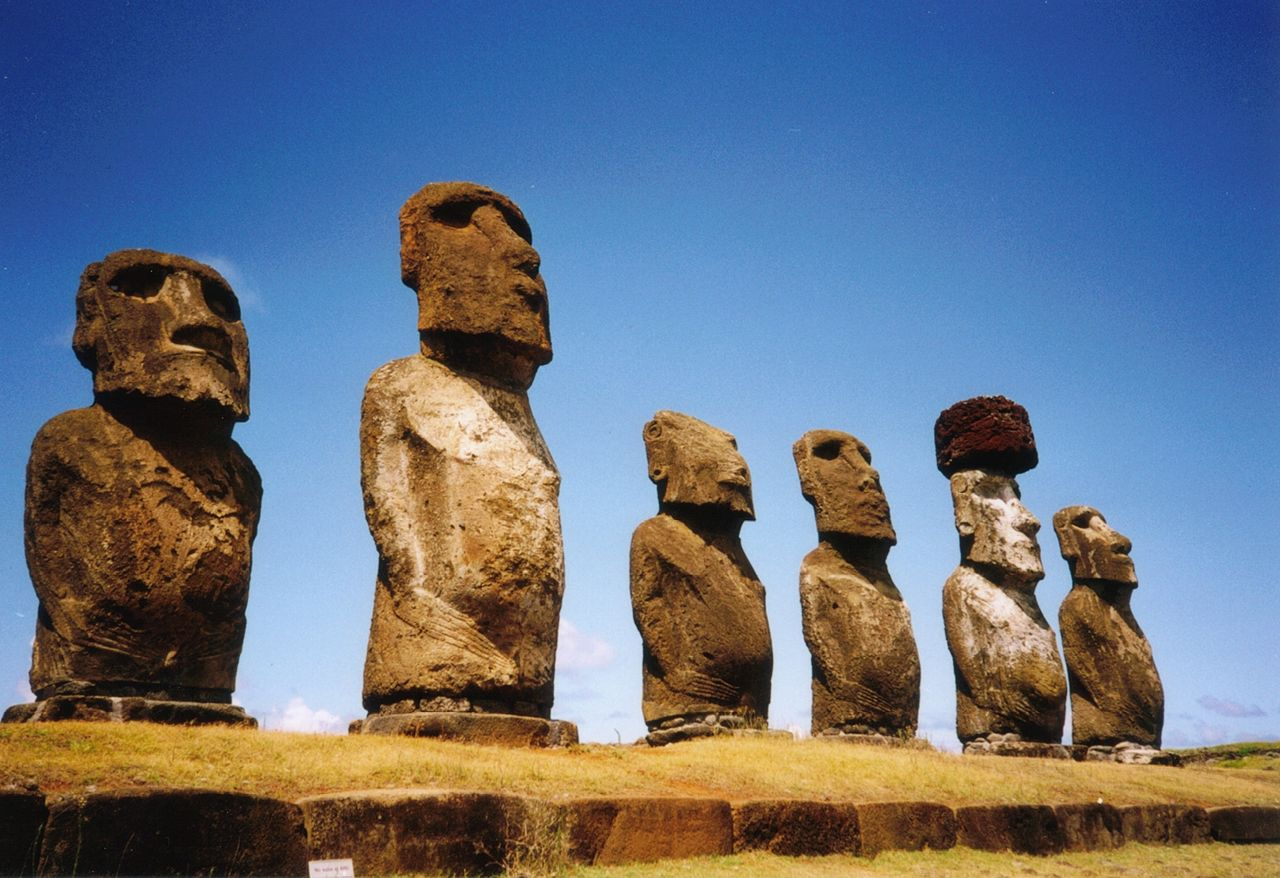
\includegraphics[height=1cm]{images/moai3.jpg}
	\caption{{\scriptsize Moai Statues}}}
	\end{subfigure}\hfill
	\begin{subfigure}{0.18\textwidth}
	\centering			\only<1-6>{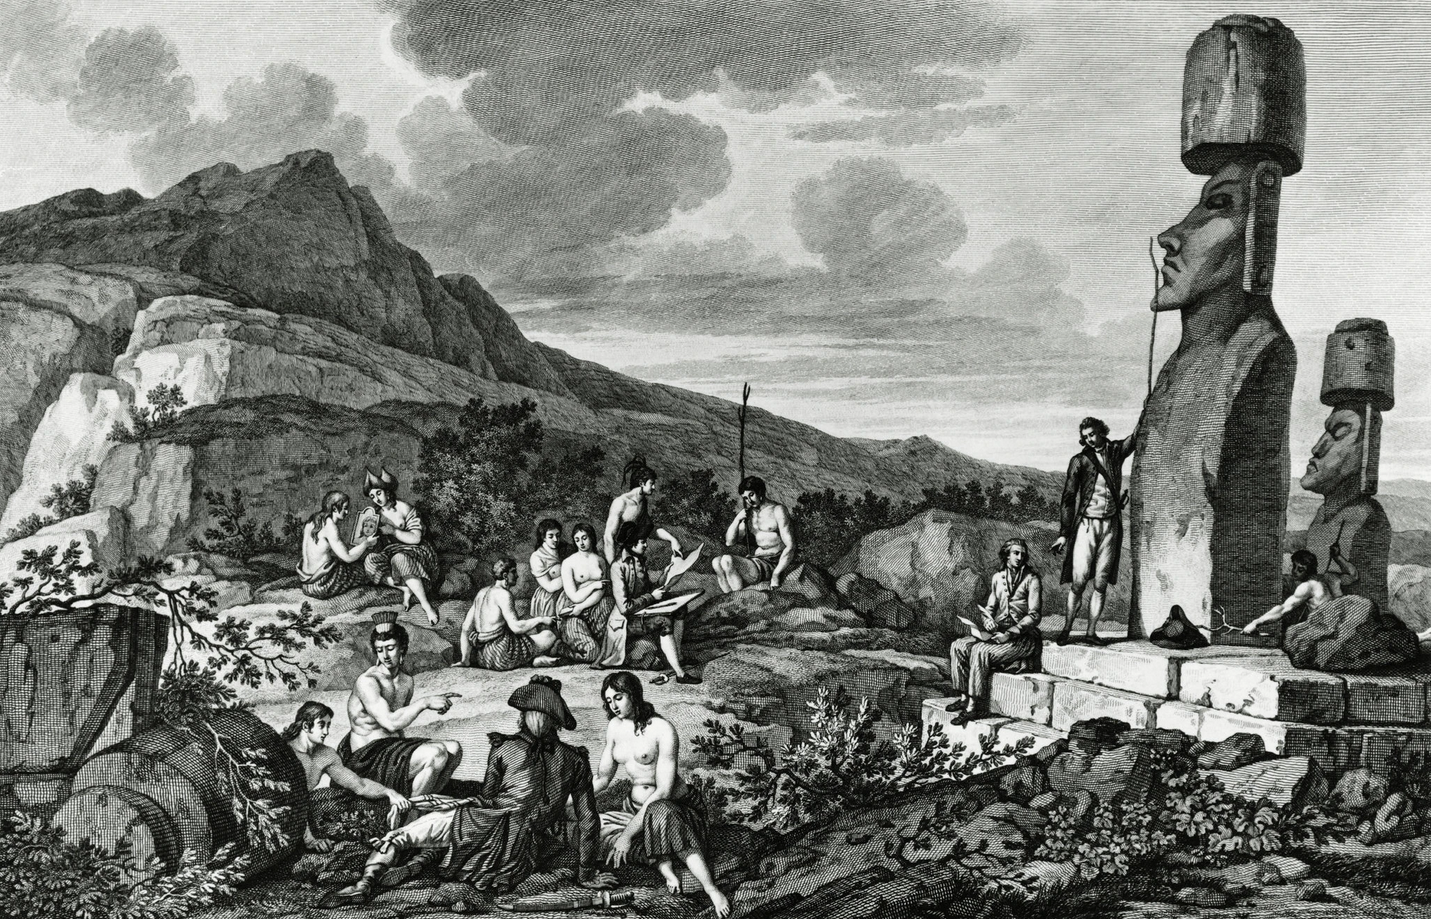
\includegraphics[height=1cm]{images/voyages.png}
	\caption{{\scriptsize European Contact}}}
	\end{subfigure}
\end{figure}
%
\begin{figure}
	\centering
	\only<1>{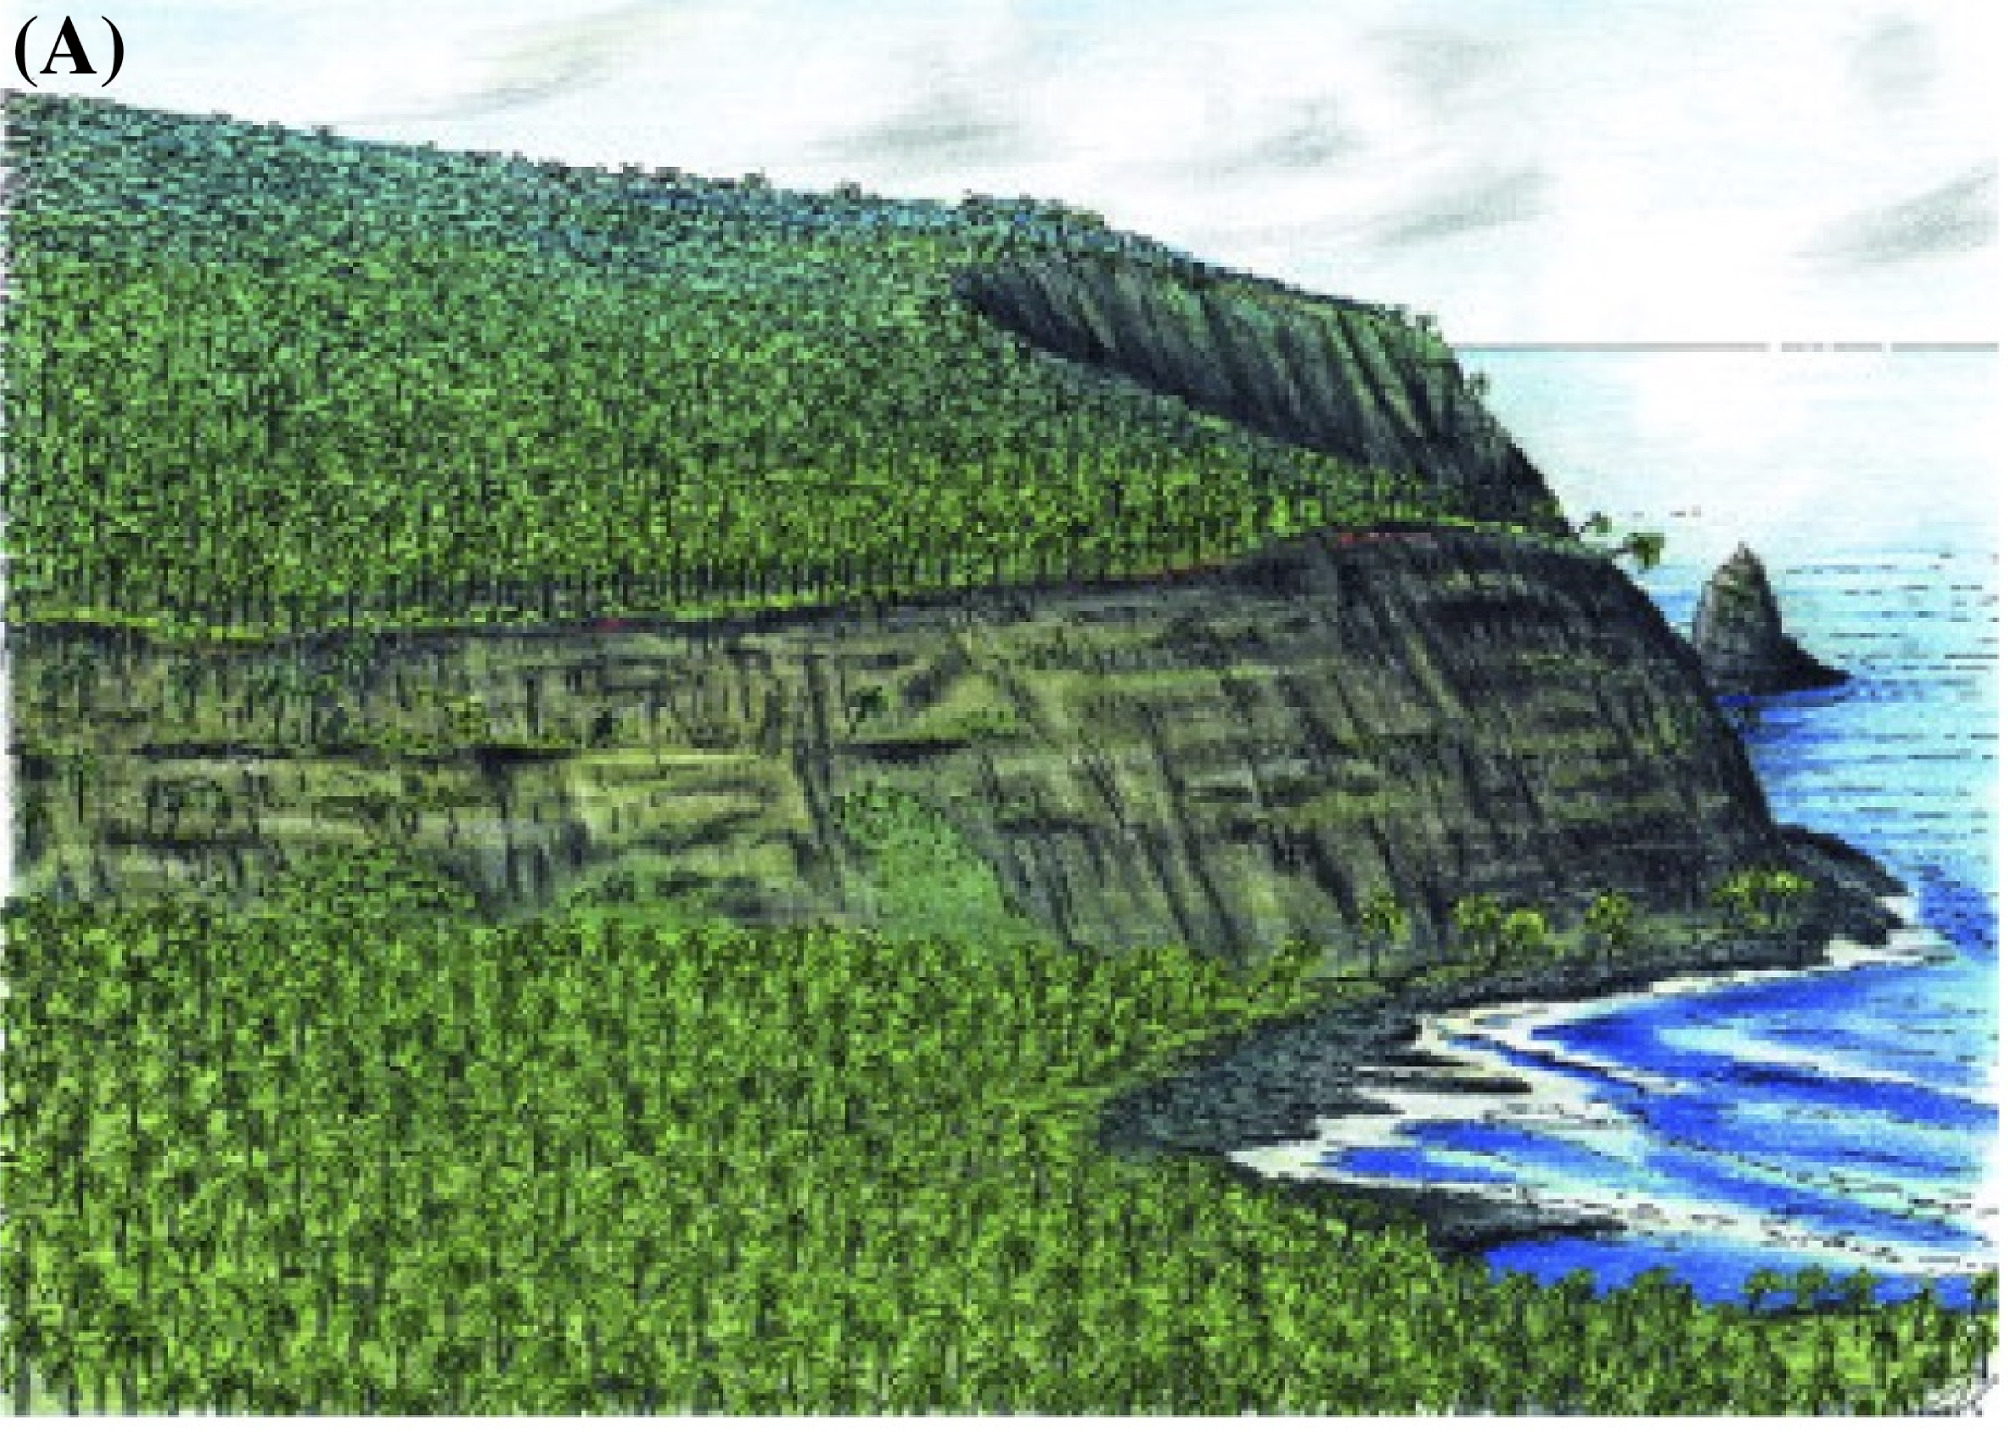
\includegraphics[height=4cm]{images/ForestGerdCloseRull2020.jpg}
	\caption{Palm Forest}
	\flushright{\tiny Artisitc Rendering, \citet{Rull2020}}
	}	
	\only<2>{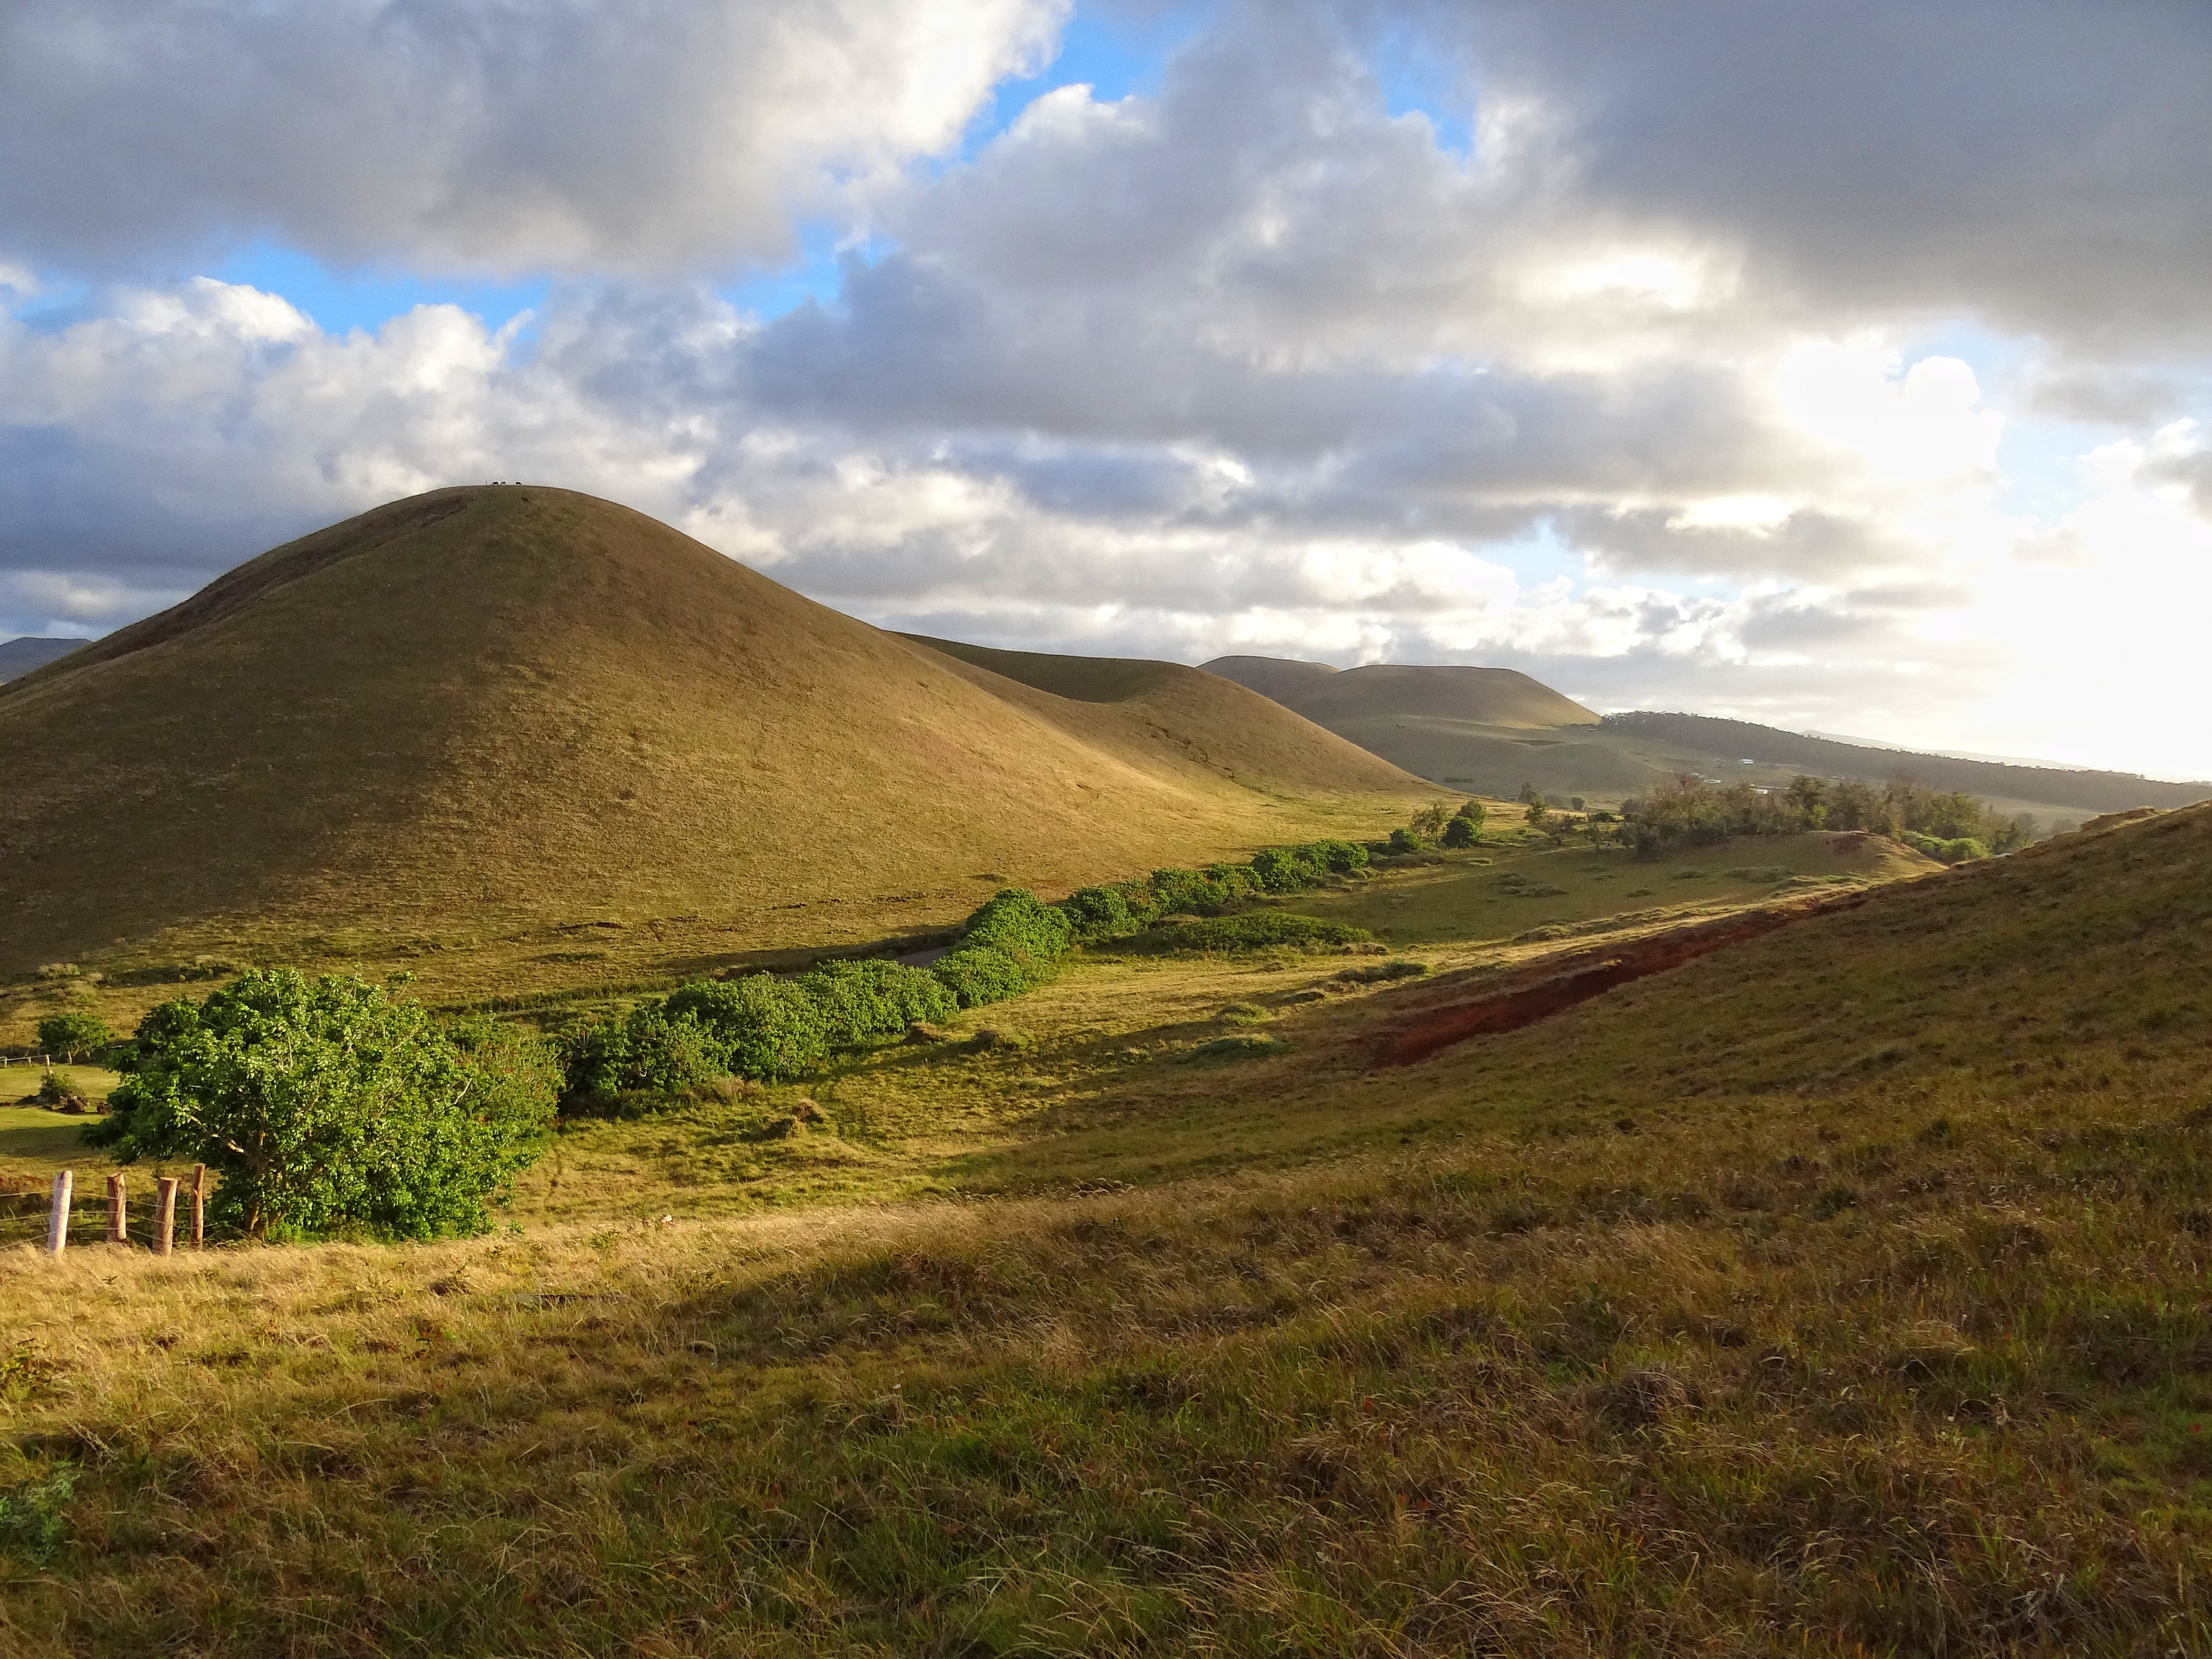
\includegraphics[height=4cm]{images/Rapa-Nui-Landscape.jpg}
	\caption{Deforestation}
	\flushright{\tiny Modern Day Image \url{en.wikipedia.org/wiki/Easter_Island}}
	}
	\only<3>{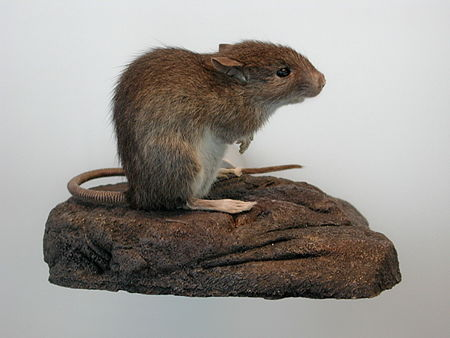
\includegraphics[height=4cm]{images/Pacific_rat.jpg}
	\caption{Pacfic Rats}
	\flushright{\tiny \url{de.wikipedia.org/wiki/Pazifische_Ratte}}
	}
	\only<4>{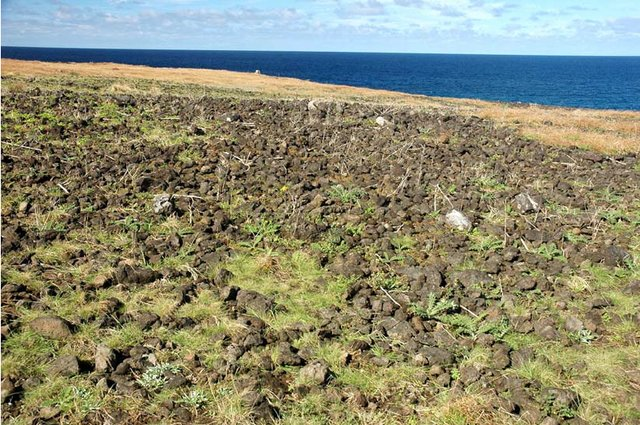
\includegraphics[height=4cm]{images/lithicMulching.jpg}
		\caption{Agriculture}
		 	\flushright{\tiny \citet{Hunt2009}}}
	\only<5>{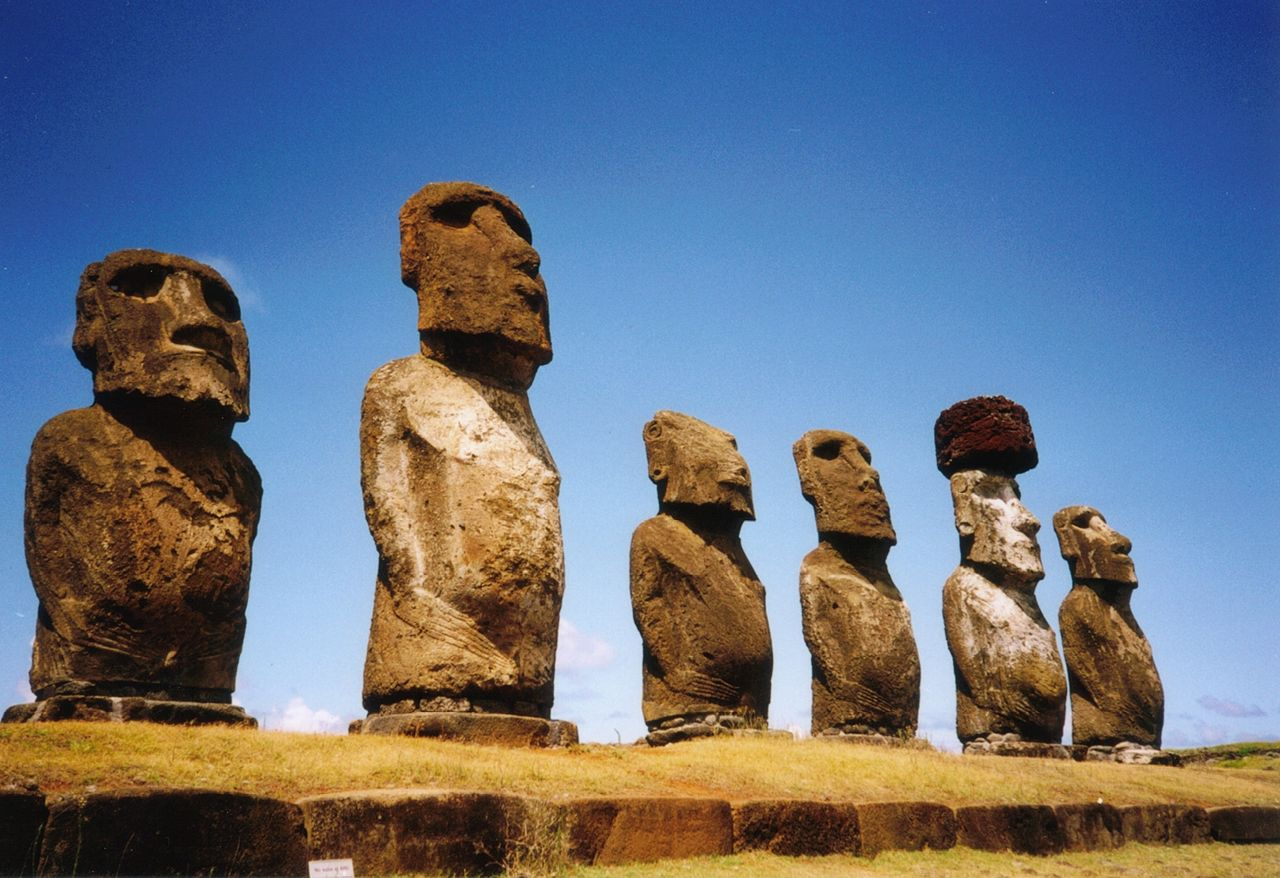
\includegraphics[height=4cm]{images/moai3.jpg}
		\caption{Moai Statues}
	\flushright{\tiny \url{https://nl.wikipedia.org/wiki/Moai}}
	}
	\only<6>{
		\begin{columns}
			\centering
			\begin{column}{0.4\textwidth}
				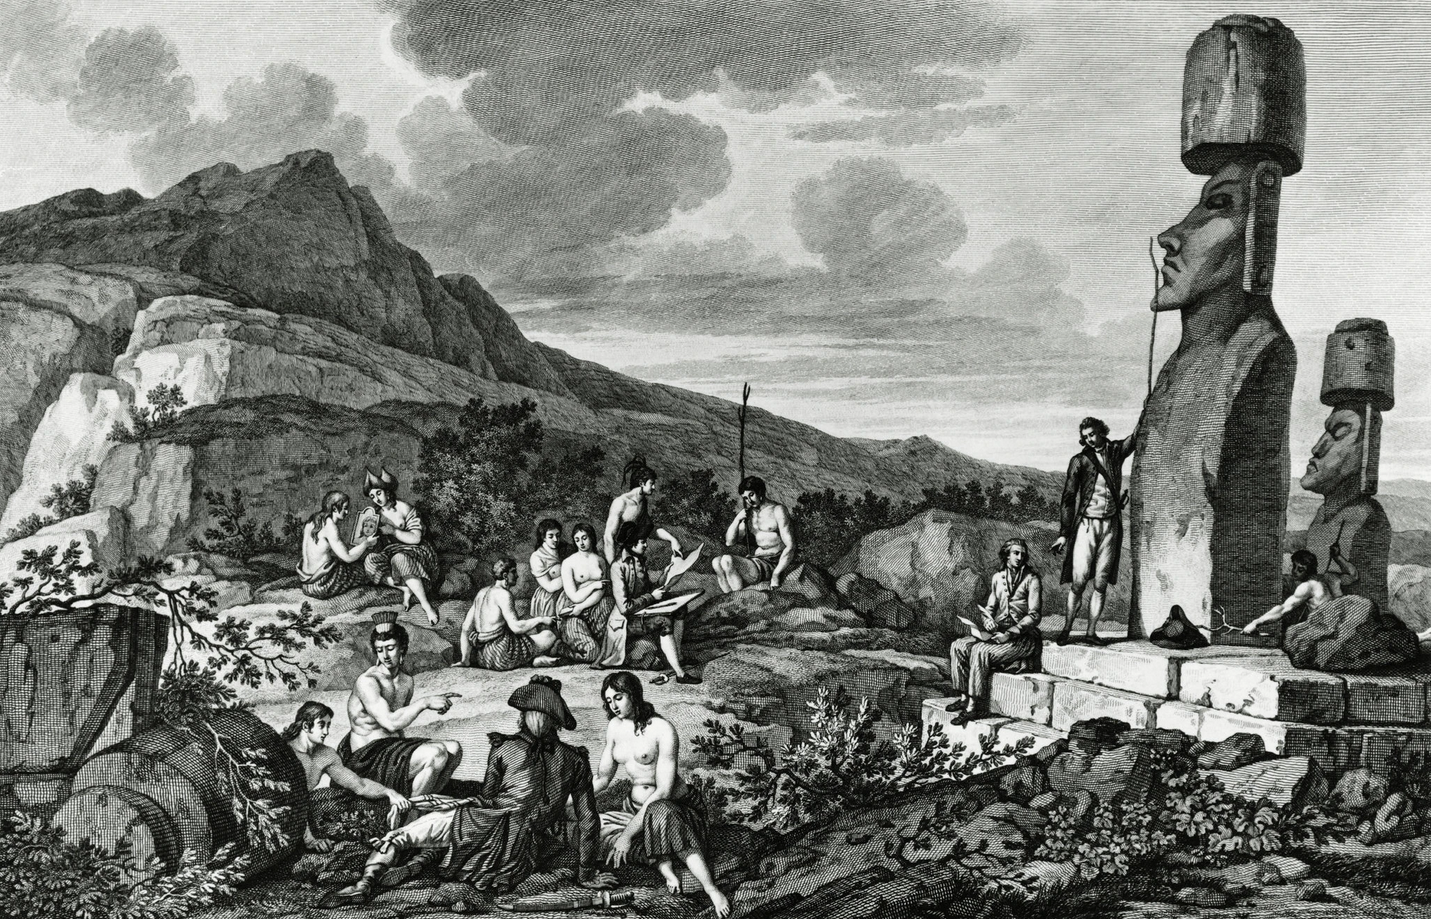
\includegraphics[height=4cm]{images/voyages.png}
				\caption{European Contact}
			\end{column}
			\begin{column}{0.4\textwidth}
			
				\textbf{Observations:} \vspace{0.2cm}
%				\begin{columns}
%					\begin{column}{0.3\textwidth}
%						\begin{itemize}
%							\item Advanced civilisation 
%							\item Initially Dense Forest
%						\end{itemize}
%					\end{column}
%					\begin{column}{0.1\textwidth}\centering
%						\textbf{\Huge \lightning}
%					\end{column}
%					\begin{column}{0.6\textwidth}
%						\begin{itemize}
%							\item Declining population number, 
%							\item Moai on the floor, 
%							\item Barren Island
%						\end{itemize}
%				\end{column}
%				\end{columns}
			\begin{itemize}
				\item Advanced civilisation 
				\item Initially dense forest
				\item Barren island
				\item Declining population number
				\item Moai lying on the ground
			\end{itemize}
			\end{column}
		\end{columns}
	\flushleft{\tiny  \url{www.nytimes.com/2017/10/12/science/easter-island-dna-south-america.html}}
	}

		
%	\only<7>{\centering \textbf{Observations}\begin{columns}
%			\begin{column}{0.4\textwidth}
%				\begin{itemize}
%					\item Dense Forest before human arrival
%					\item Built Moai Statues
%					\item Used Advanced farming techniques
%				\end{itemize}
%			\end{column}
%		\begin{column}{0.05\textwidth}
%			\centering
%			{\Huge\lightning}
%		\end{column}
%			\begin{column}{0.4\textwidth}
%				\begin{itemize}
%					\item Only a few thousand people ($100$ in $1860\, {\rm A.D.}$) 
%					\item Moai Statues on the floor
%					\item  Barren Island (no large vegetation)
%				\end{itemize}
%				
%			\end				\end{columns}{column}
%		\end{columns}}
\end{figure}
\begin{figure}
	\centering

\only<1-3>{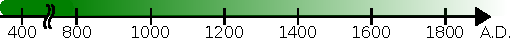
\includegraphics[width=0.6\linewidth]{images/timeline}}
\only<4,5>{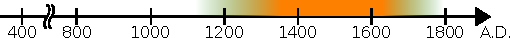
\includegraphics[width=0.6\linewidth]{images/timeline_agric}}	\only<6>{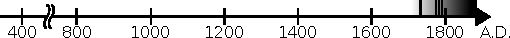
\includegraphics[width=0.6\linewidth]{images/timeline_european}}
\end{figure}
\end{frame}

\begin{frame}{The Mystery -- Two Major Narratives}
\begin{columns}
		\begin{column}{0.4\textwidth}
		\textbf{Ecocidal View}\\ \citet{Brander1998}, \citet{Diamond2011}, \citet{Bahn2017} \\ \ \\
		Early arrival, \\ 
		\ra Population grows slowly exponentially, \\
		\ra Intensification of agriculture and deforestation, \\
		\ra Population reaches $6k$ to $20k$ people in 17th century, \\ 
		\ra Overexploitation of resources and conflict (Malthusian catastrophe),
		\\
		\ra `Collapse' prior to European contact
	\end{column}


	\begin{column}{0.4\textwidth}
		\textbf{Genocidal View}\\ \citet{Peiser2005}, \citet{Hunt2007}, \citet{Basener2008}\\ \  \\
		Late arrival, \\
		\ra Population grows quickly and then remains constant at $4k$ people, \\
		\ \\
		\ra Rats cause deforestation, \\
		\ra Humans resilient, \\
		 \ \\
		\ra European contact triggers decline due to slave trades and diseases \\
		 \ \\
		 \ \\
		 

	\end{column}

\end{columns}
\centering
{\color{red}$\Downarrow$}\\
{\color{red} Population dynamics?}
\end{frame}


%
%\begin{frame}{The Mystery -- Two Narratives}
%\begin{columns}
%	\begin{column}{0.2\textwidth}
%		\ \\ \ \\ \ \\
%		\begin{itemize}
%			\item Arrival
%			\item Growth of Human Population
%			\item Deforestation
%			\item Agriculture intesification
%			\item Population size peak
%			\item Aftermath
%		\end{itemize}
%	\end{column}
%	\begin{column}{0.4\textwidth}
%		\textbf{Genocidal View}\\ \citet{Hunt2007} \\ \ 
%		\begin{itemize}
%			\item $1200\, {\rm A.D.}$
%			\item Fast 
%			\item Because rat population sky-rockets
%			\item immediately, after $1200\, {\rm A.D.}$
%			\item at $4$ k people in $14th century$
%			\item Civilisation resilient to environmental degradation, but `genocide' due to European diseases and slave trade
%		\end{itemize}
%	\end{column}
%	\begin{column}{0.4\textwidth}
%		\textbf{Ecocidal View}\\ \citet{Diamond2011}, \citet{Bahn2017}, \citet{Brander1998}
%		\begin{itemize}
%			\item before $1000\,{\rm A.D.}$
%			\item Slow
%			\item Humans started deforesting and lived off the natural resources (provided by trees)
%			\item only after $1200\, {\rm A.D.}$
%			\item at $6-20$ k people in $17$th century
%			\item Overexploitation and erosion, resources scarce, potential conflict, `collapse' (Malthusian Catastrophe) prior to European contact
%		\end{itemize}
%	\end{column}
%\end{columns}
%\end{frame}
